\documentclass[a4paper,12pt]{article}
\usepackage{amsmath}
\usepackage{hyperref}
\usepackage{graphicx}
\usepackage{float}
\usepackage{subcaption}
\usepackage{listings}
\usepackage{circuitikz}
\usepackage{tikz}
\title{Lab Report2}
\author{Arnav Yadnopavit- EE24BTECH11007\\Prajwal - EE24BTECH11051}
\date{\today}

\begin{document}

\maketitle
\section*{Objective}
\begin{enumerate}
    \item Observing the RC response for the square wave input in steady and transient state
    \begin{itemize}
        \item RC==T
        \item RC$>>$T
        \item RC$<<$T
    \end{itemize}
\end{enumerate}
\section*{Apparatus}
\begin{itemize}
    \item Capacitor(1$\mu F$),Resistor(100 $\Omega$),Breadboard
    \item Cathode Ray Oscilloscope (CRO)
    \item Signal Generator (1 channel)
    \item Probes and Connecting Wires
\newpage
\end{itemize}


\section*{Procedure}
\begin{enumerate}
    \item Form a circuit using the resistor and capacitor in series 
\end{enumerate}
\begin{figure}[H]
\centering
\label{fig:my_label}
\begin{circuitikz}
\tikzstyle{every node}=[font=\LARGE]
\draw (6.5,11) to[R] (12.75,11);
\draw (11.5,11) to[C] (11.5,7.25);
\draw (12.75,7.25) to[short] (6.5,7.25);
\draw (12.5,7.25) to[short] (13,7.25);
\draw (12.25,11) to[short, -o] (13,11) ;
\draw (12.75,7.25) to[short, -o] (13.25,7.25) ;
\draw (6.75,11) to[short, -o] (6.5,11) ;
\draw (7,7.25) to[short, -o] (6.5,7.25) ;
\node [font=\normalsize] at (9.5,11.75) {R=100$\Omega$};
\node [font=\normalsize] at (6,11.5) {A};
\node [font=\normalsize] at (13,11.5) {B};
\node [font=\normalsize] at (6,6.75) {C};
\node [font=\normalsize] at (13.5,7) {D};
\node [font=\normalsize] at (6.25,9.25) {Input Signal};
\node [font=\normalsize] at (13.25,9.25) {Output Signal};
\node [font=\normalsize] at (10,9.25) {C=1$\mu$F};
\end{circuitikz}
\end{figure}
\begin{enumerate}
    \item Connect the signal generator at the input i.e, at A and ground probe at C
    \item Connect the probe of CRO at the output i.e, at B and ground probe at D.
    \item Adjust the time period and observe the reponse of RC series circuit for different time periods.
\end{enumerate}
\section*{Theory}
     \begin{itemize}
            \item From kirchhof's circuit law the governing equation is given by,
            \begin{align}
                V_{in}(t)=I(t)R+V_c(t)\\
                I(t)=C\frac{dV_c}{dt}
            \end{align}
            finally,
            \begin{align}
                V_{in}(t)=RC\frac{dV_c}{dt}+V_c(t)\label{3}
            \end{align}
        \item We have to the equation \eqref{3} in two parts
        \begin{enumerate}
            \item During Charging ($V_{in}(t)=V_{high}$)\\
                    \begin{itemize}
                    \item The differential equation becomes:
                    \begin{align}
                         V_{high}=RC\frac{dV_c}{dt}+V_c(t)
                    \end{align}
                    \item Solve using the integrating factor method or by inspection:
                    \begin{align}
                        V_c(t)=V_{final}+(V_{initial}-V_{final})e^{-\frac{t}{\tau}}
                    \end{align}
                    \item $V_{final}=V_{high}$
                    \item $\tau$=RC
                    \end{itemize}
            \item During Discharging ($V_{in}(t)=V_{low}$)\\
                    \begin{itemize}
                    \item The differential equation becomes:
                    \begin{align}
                         V_{low}=RC\frac{dV_c}{dt}+V_c(t)
                    \end{align}
                    \item Solve using the integrating factor method or by inspection:
                    \begin{align}
                        V_c(t)=V_{final}+(V_{initial}-V_{final})e^{-\frac{t}{\tau}}
                    \end{align}
                    \item $V_{final}=V_{low}$
                    \item $\tau$=RC
                    \end{itemize}
        \end{enumerate}
    \end{itemize}
    \newpage
\section{Observing RC response in steady state}
\subsection{When $\tau$=T}
\begin{itemize}
    \item \textbf{Figures}
    \begin{figure}[H]
    \centering
    \begin{subfigure}{0.48\textwidth}
        \centering
        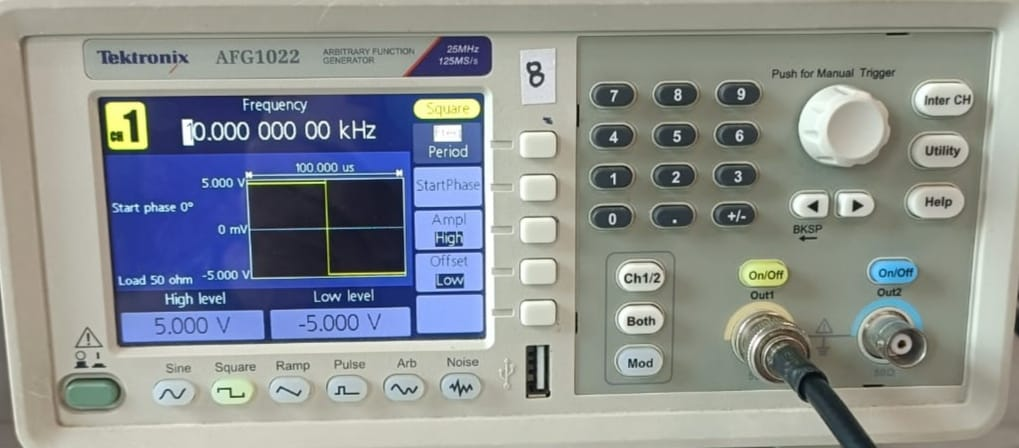
\includegraphics[height=5cm]{figs/inputrc==t.jpeg}
    \end{subfigure}
    \hspace{0.04\textwidth} % Adjust the spacing as needed 
    \begin{subfigure}{0.48\textwidth}
        \centering
        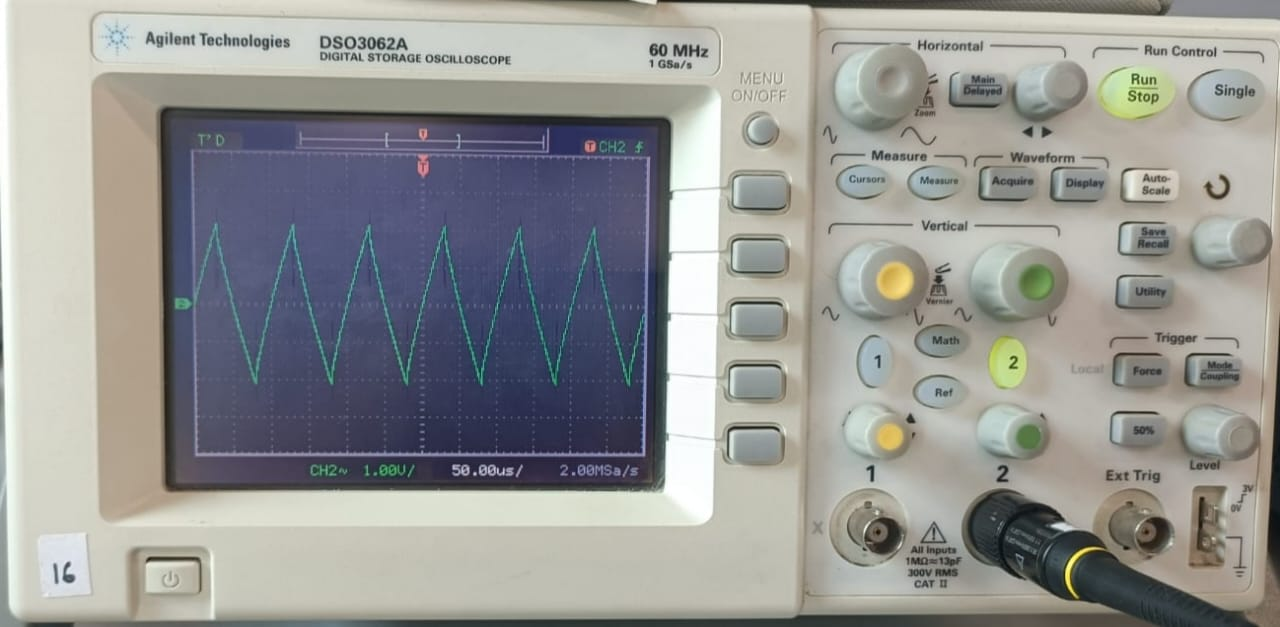
\includegraphics[height=5cm]{figs/outputrc==t.jpeg}
    \end{subfigure}
    \item \textbf{Observation}
    \begin{itemize}
        \item The capacitor never charges or discharges completely. it just exponentially charges and discharges in every half cycle
        \item It never reaches the $V_{high}$ or $V_{low}$
        \item The capacitor voltage will appear as a smoothed waveform, lagging behind the input and transitioning exponentially.
    \end{itemize}
\end{figure}
\end{itemize}
\newpage


\subsection{When $RC\ll T$}
\begin{itemize}
    \item \textbf{Figures}
    \begin{figure}[H]
    \centering
    \begin{subfigure}{0.48\textwidth}
        \centering
        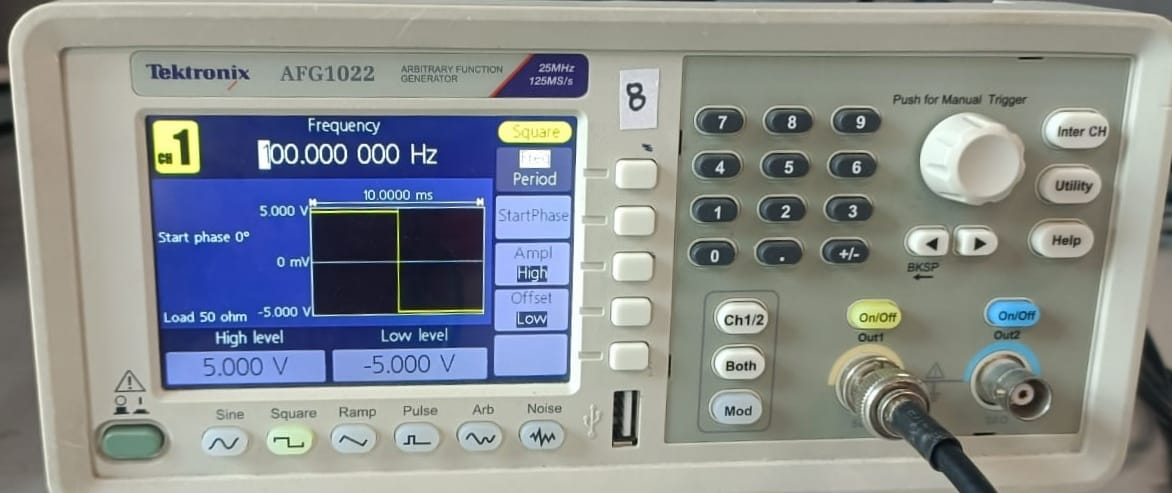
\includegraphics[height=5cm]{figs/inputrc<<t.jpeg}
    \end{subfigure}
    \hspace{0.04\textwidth} % Adjust the spacing as needed 
    \begin{subfigure}{0.48\textwidth}
        \centering
        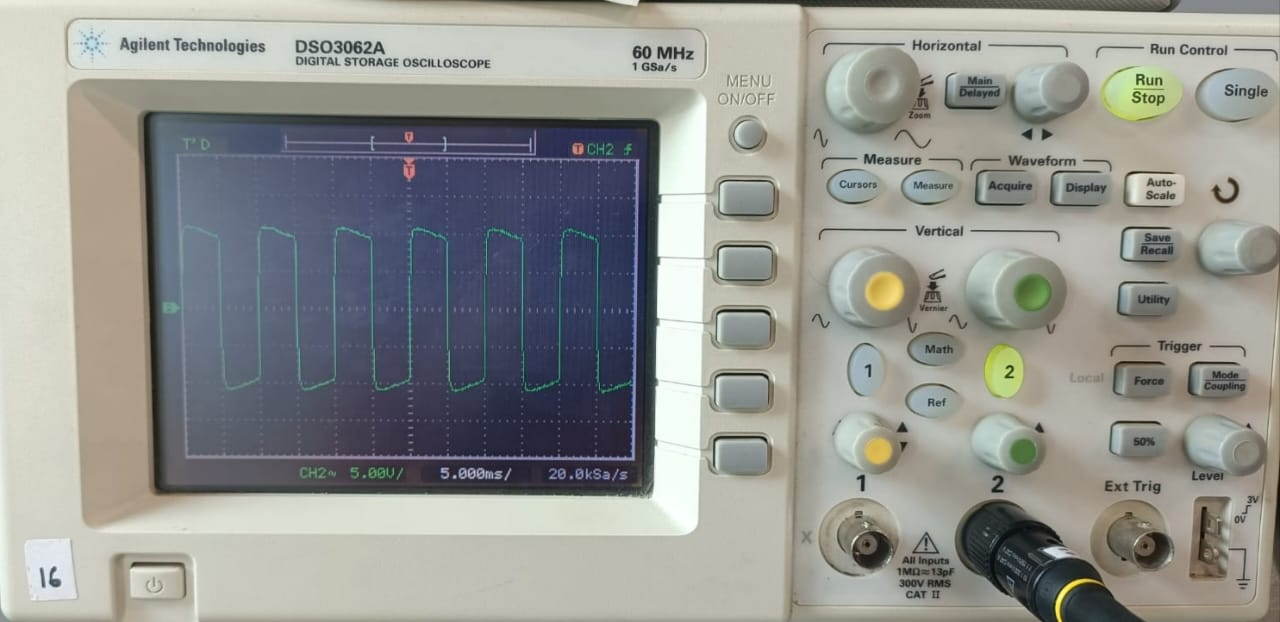
\includegraphics[height=5cm]{figs/outputrc<<t.jpeg}
    \end{subfigure}
    \item \textbf{Observation}
    \begin{itemize}
        \item The capacitor gets fully charged and fully discharged in each cycle as $RC\ll T$
        \item It almost follows the square wave form
    \end{itemize}
\end{figure}
\end{itemize}
\newpage

\subsection{When $RC\gg T$}
\begin{itemize}
    \item \textbf{Figures}
    \begin{figure}[H]
    \centering
    \begin{subfigure}{0.48\textwidth}
        \centering
        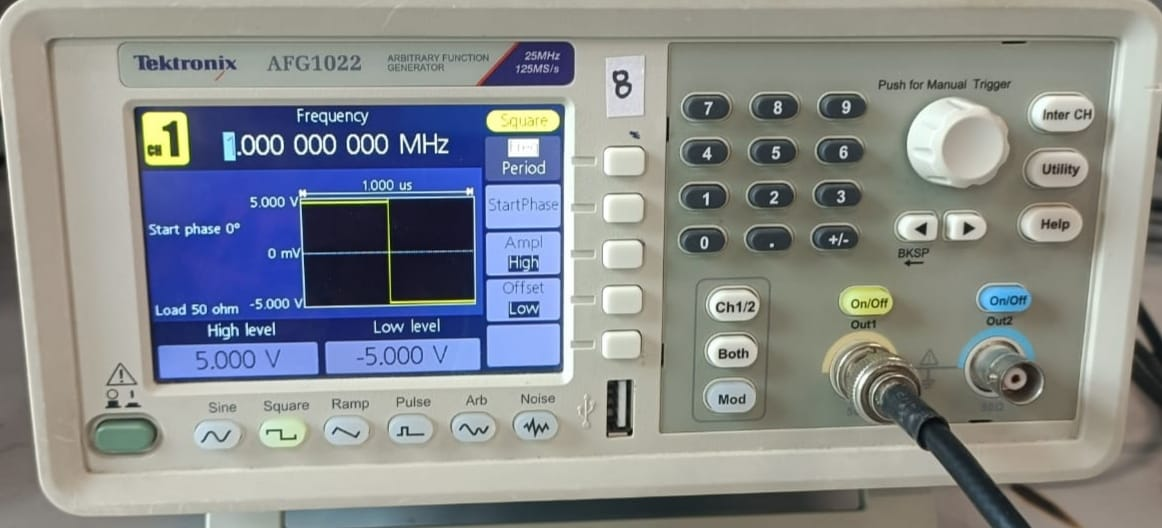
\includegraphics[height=5cm]{figs/inputrc>>t.jpeg}
    \end{subfigure}
    \hspace{0.04\textwidth} % Adjust the spacing as needed 
    \begin{subfigure}{0.48\textwidth}
        \centering
        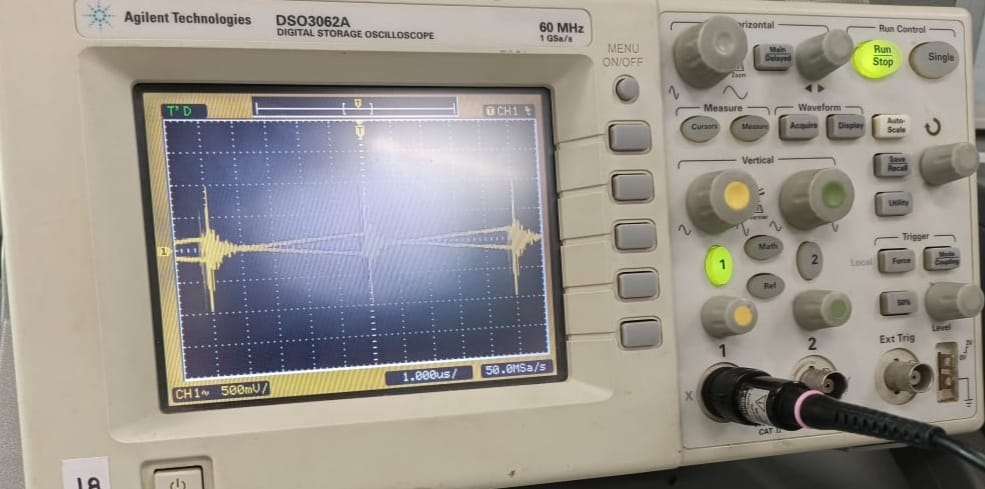
\includegraphics[height=5cm]{figs/outputrc>>t.jpeg}
    \end{subfigure}
    \item \textbf{Observation}
    \begin{itemize}
        \item The capacitor in the circuit acts as a low-pass filter.
        \item The capacitor is not able to pick up with the rapid change between +V and -V of the square wave.
    \end{itemize}
\end{figure}
\end{itemize}
\newpage

\section{Observing RC response in transition state}
\textbf{Procedure}
\begin{itemize}
    \item Same as previously described but now we will pass only for 5 time periods from function generator
    \item We have set the CRO to one time event capture mode
\end{itemize}
\subsection{When $\tau$=T}
\begin{itemize}
    \item \textbf{Figures}
    \begin{figure}[H]
    \centering
    \begin{subfigure}{0.48\textwidth}
        \centering
        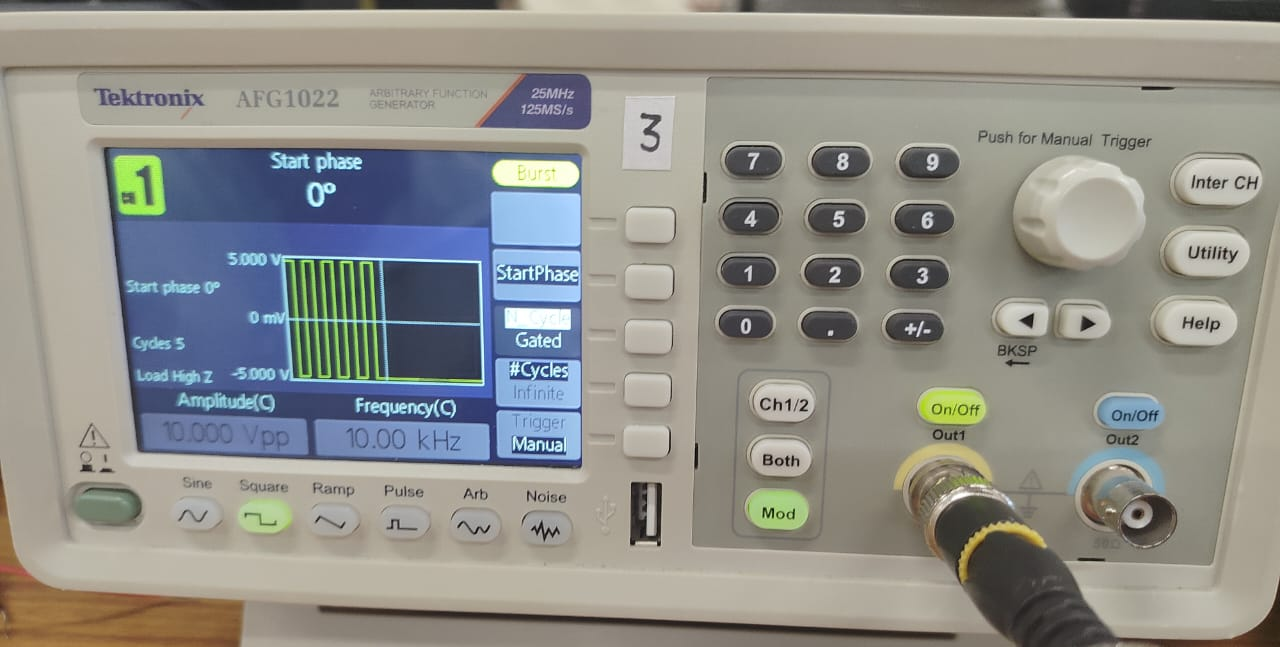
\includegraphics[height=5cm]{figs/transinputrc==t.jpeg}
    \end{subfigure}
    \hspace{0.04\textwidth} % Adjust the spacing as needed 
    \begin{subfigure}{0.48\textwidth}
        \centering
        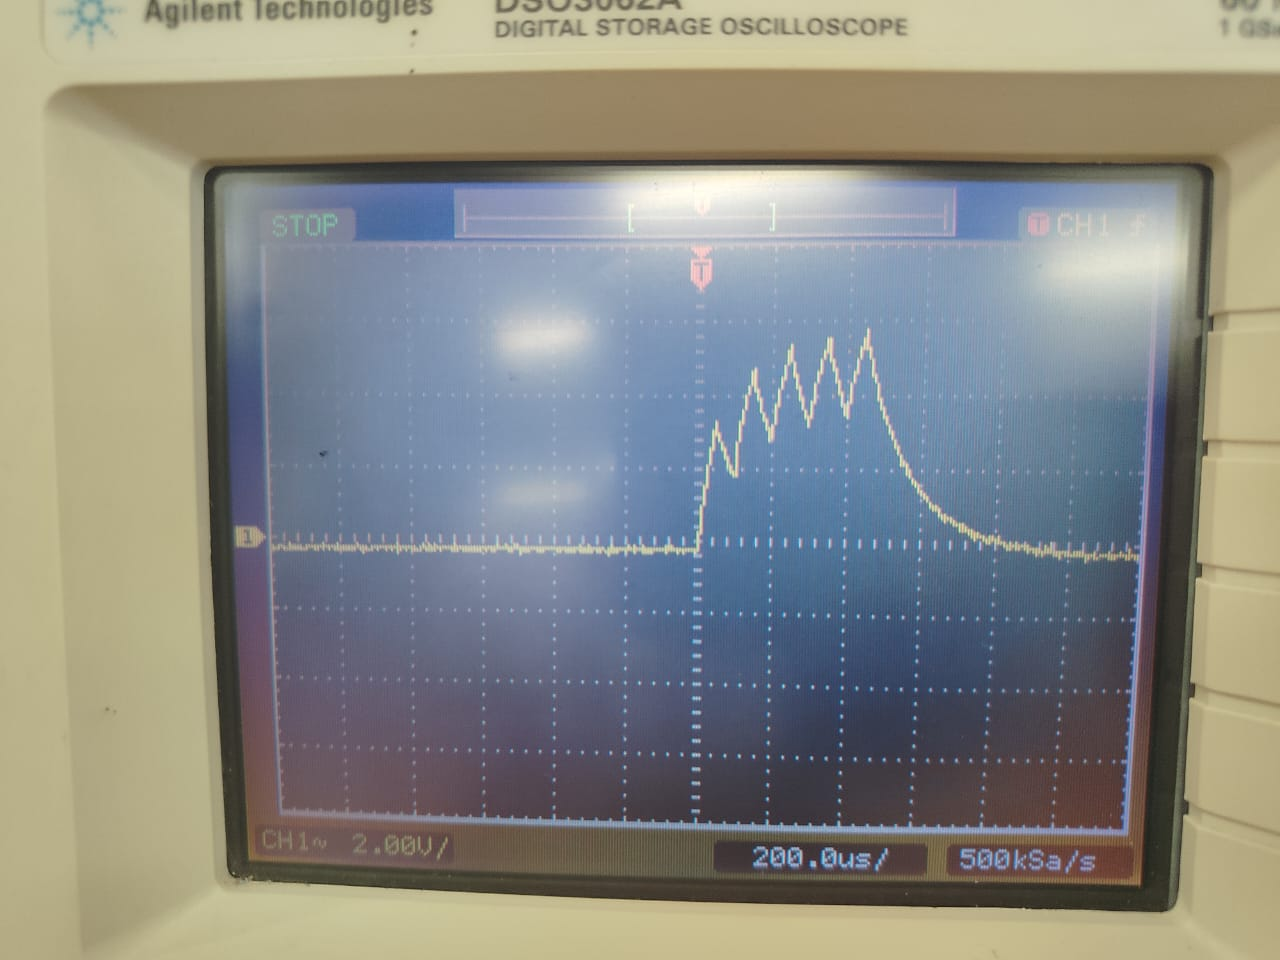
\includegraphics[height=5cm]{figs/transoutputrc==t.jpeg}
    \end{subfigure}
    \item \textbf{Observation}
    \begin{itemize}
        \item The capacitor never charges or discharges completely. it just exponentially charges and discharges in every half cycle
        \item initially it charges and in the second half it discharges but not compltely
        \item and the cycle goes on continuing untill steady state
    \end{itemize}
\end{figure}
\end{itemize}
\newpage


\subsection{When $RC\ll T$}
\begin{itemize}
    \item \textbf{Figures}
    \begin{figure}[H]
    \centering
    \begin{subfigure}{0.48\textwidth}
        \centering
        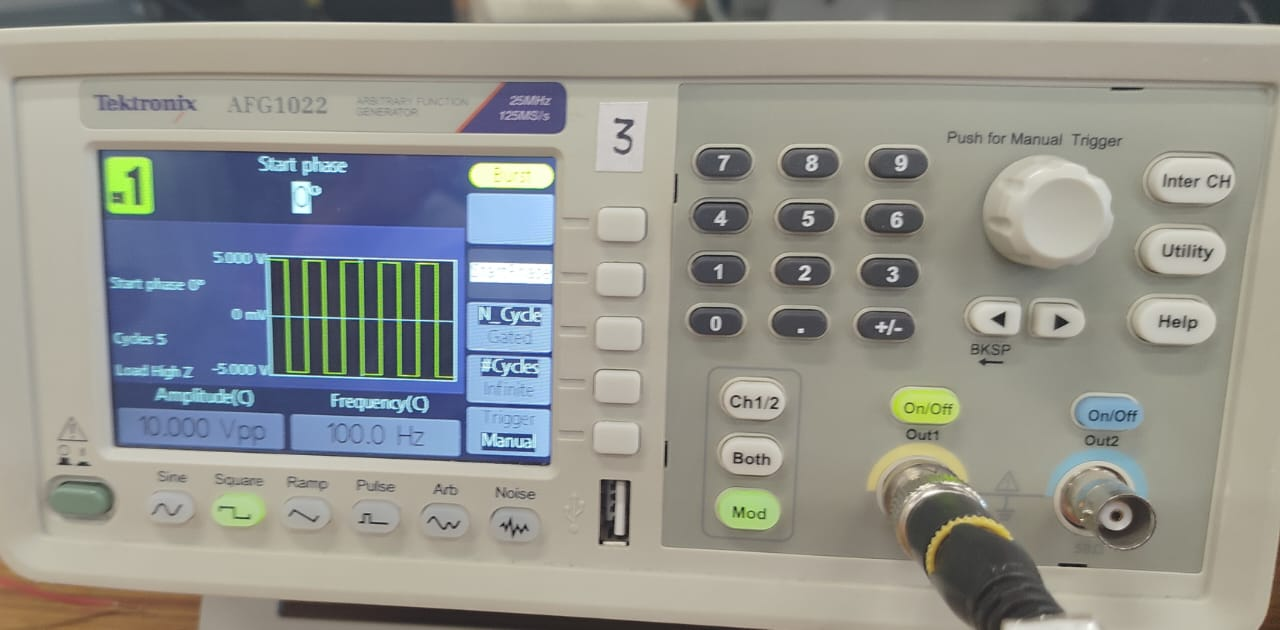
\includegraphics[height=5cm]{figs/transinputrc<<t.jpeg}
    \end{subfigure}
    \hspace{0.04\textwidth} % Adjust the spacing as needed 
    \begin{subfigure}{0.48\textwidth}
        \centering
        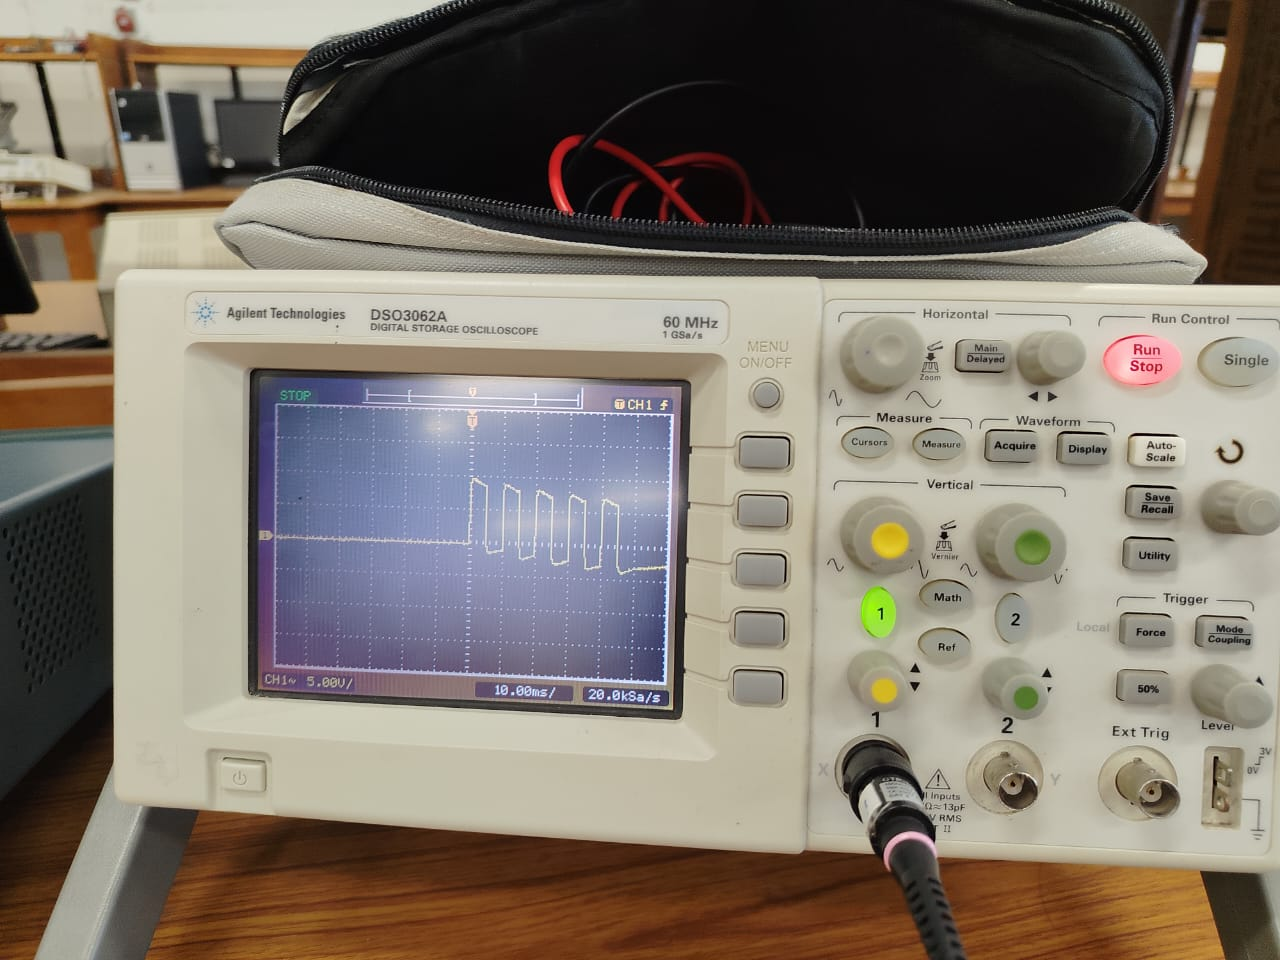
\includegraphics[height=5cm]{figs/transoutputrc<<t.jpeg}
    \end{subfigure}
    \item \textbf{Observation}
    \begin{itemize}
        \item The capacitor gets fully charged and fully discharged in each cycle as $RC\ll T$
        \item It almost follows the square wave form
    \end{itemize}
\end{figure}
\end{itemize}
\newpage

\subsection{When $RC\gg T$}
\begin{itemize}
    \item \textbf{Figures}
    \begin{figure}[H]
    \centering
    \begin{subfigure}{0.48\textwidth}
        \centering
        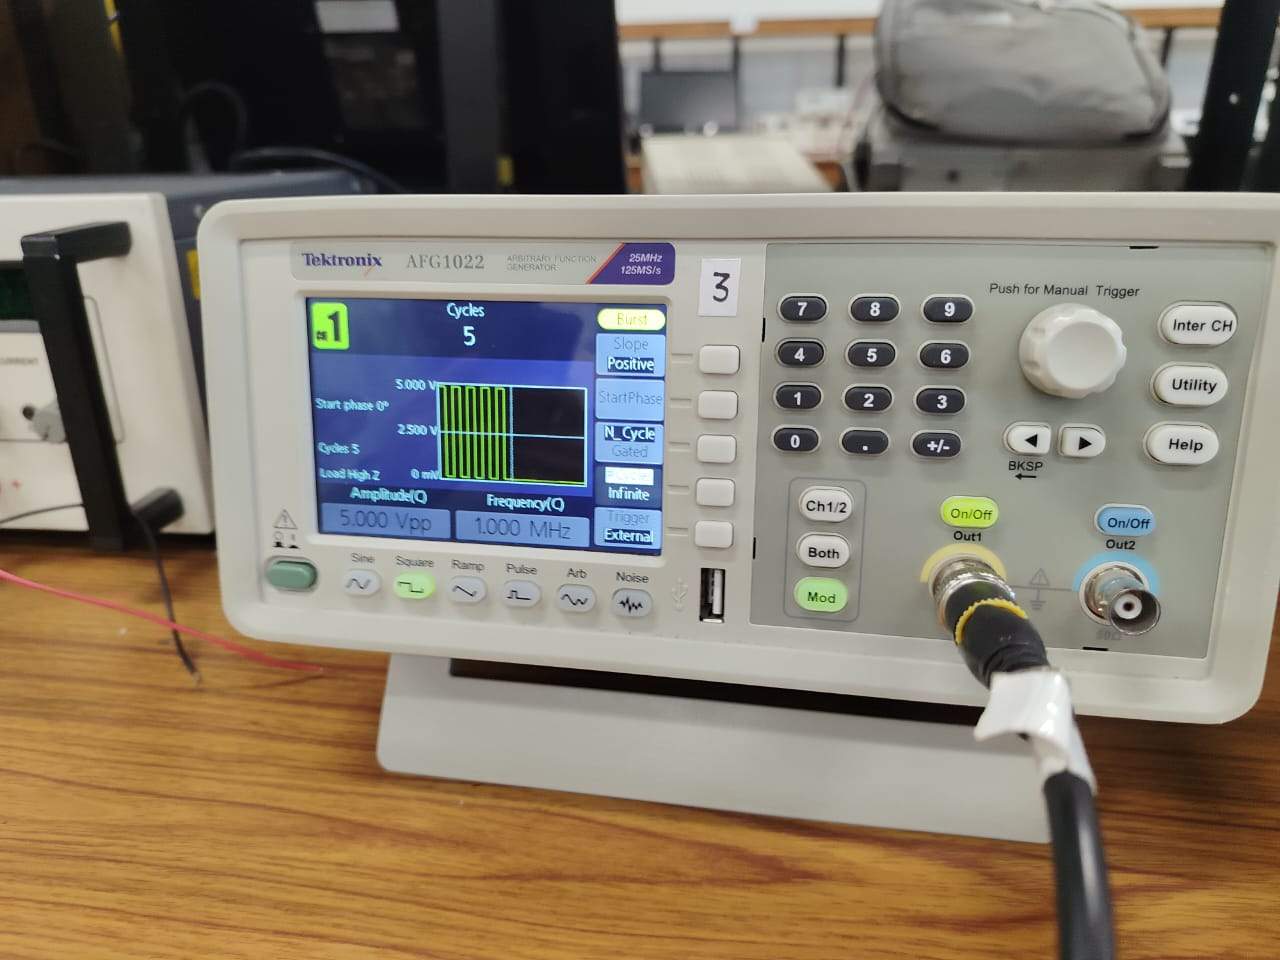
\includegraphics[height=5cm]{figs/transinputrc>>t.jpeg}
    \end{subfigure}
    \hspace{0.04\textwidth} % Adjust the spacing as needed 
    \begin{subfigure}{0.48\textwidth}
        \centering
        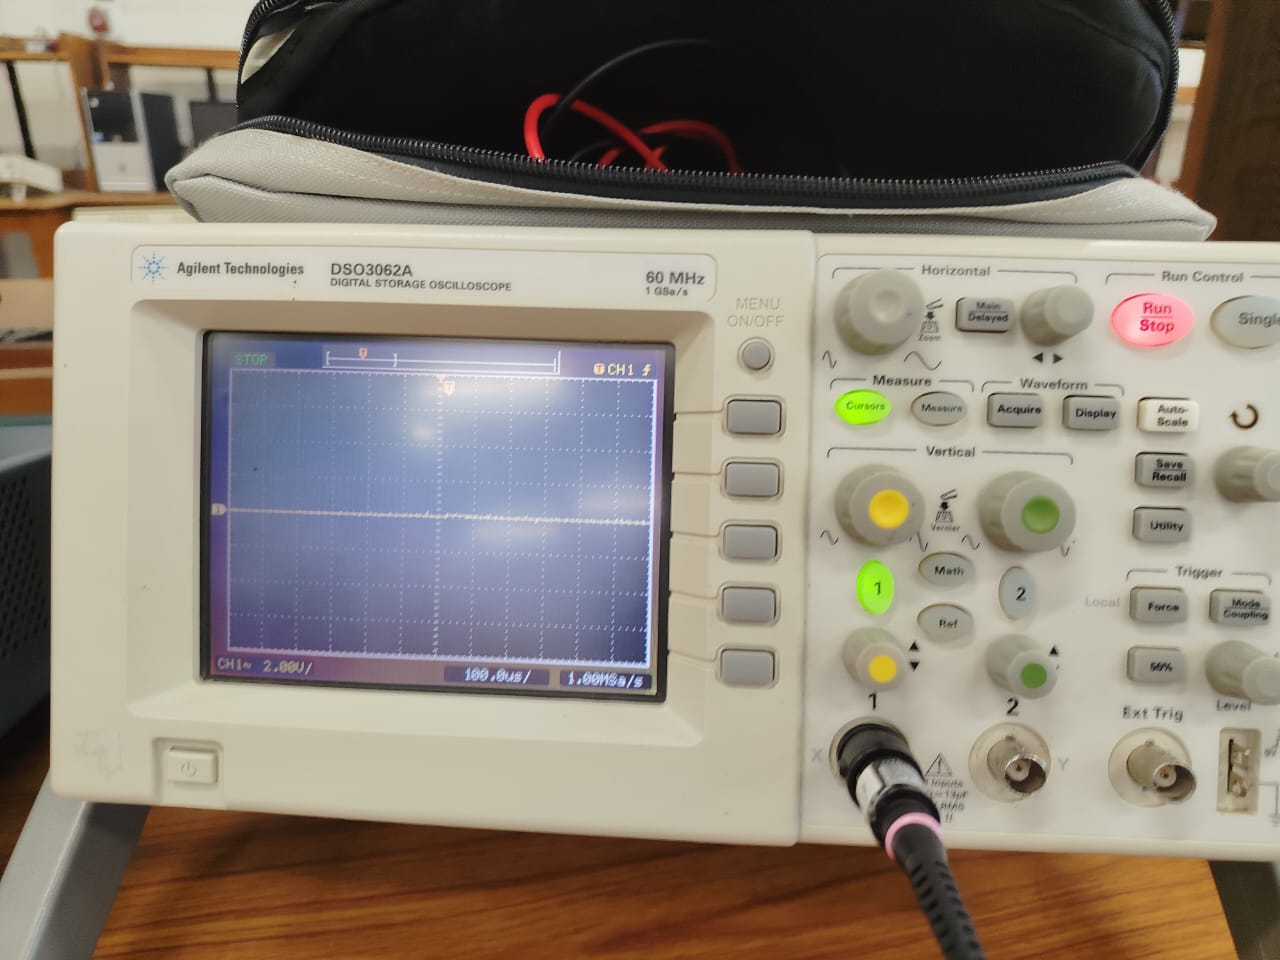
\includegraphics[height=5cm]{figs/transoutputrc>>t.jpeg}
    \end{subfigure}
    \item \textbf{Observation}
    \begin{itemize}
        \item Initially the capacitor is not able to pick up with change in square waveform  
        \item niether it get charged nor discharged hence it appeare to be flat
    \end{itemize}
\end{figure}
\end{itemize}
\newpage
\centering{Thank You}
\end{document}
